\documentclass[12pt]{standalone}
\usepackage{tikz}
\usetikzlibrary{calc,arrows,positioning}

\begin{document}

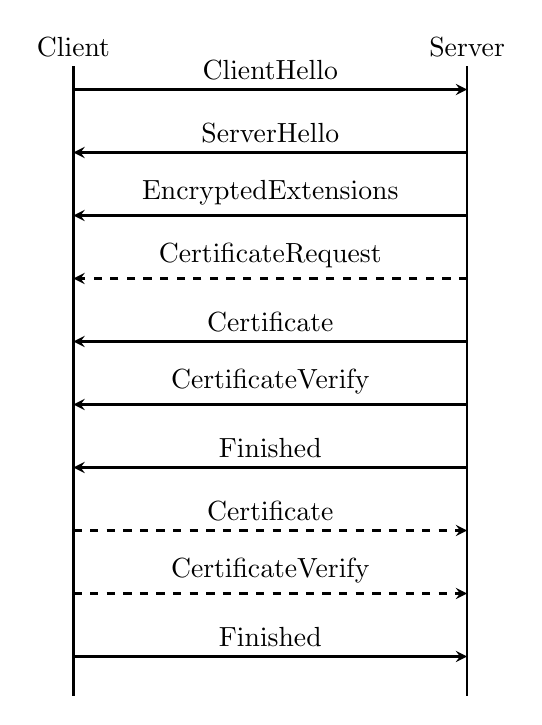
\begin{tikzpicture}
	\tikzstyle{block} = [text width=11cm]
	\coordinate (ClientTop) at (0,0);
	\coordinate[label=Client] (ClientBottom) at (0,8);
	\coordinate (ServerTop) at (5,0);
	\coordinate[label=Server] (ServerBottom) at (5,8);

	\coordinate[below=.3cm of ClientBottom] (A);
	\coordinate[below=.3cm of ServerBottom] (B);
	\coordinate[below=.8cm of B] (C);
	\coordinate[below=.8cm of A] (D);
	\coordinate[below=.8cm of C] (E);
	\coordinate[below=.8cm of D] (F);
	\coordinate[below=.8cm of E] (G);
	\coordinate[below=.8cm of F] (H);
	\coordinate[below=.8cm of G] (I);
	\coordinate[below=.8cm of H] (J);
	\coordinate[below=.8cm of I] (K);
	\coordinate[below=.8cm of J] (L);
	\coordinate[below=.8cm of K] (M);
	\coordinate[below=.8cm of L] (N);
	\coordinate[below=.8cm of N] (O);
	\coordinate[below=.8cm of M] (P);
	\coordinate[below=.8cm of O] (Q);
	\coordinate[below=.8cm of P] (R);
	\coordinate[below=.8cm of Q] (S);
	\coordinate[below=.8cm of R] (T);

	\draw[thick] (ClientTop)--(ClientBottom);
	\draw[thick] (ServerTop)--(ServerBottom);

	\draw[->,>=stealth,thick] (A) -- (B)  node[midway,sloped,above] {ClientHello};
	\draw[->,>=stealth,thick] (C) -- (D)  node[midway,sloped,above] {ServerHello};
	\draw[->,>=stealth,thick] (E) -- (F)  node[midway,sloped,above] {EncryptedExtensions};
	\draw[->,>=stealth,thick,dashed] (G) -- (H)  node[midway,sloped,above] {CertificateRequest};
	\draw[->,>=stealth,thick] (I) -- (J)  node[midway,sloped,above] {Certificate};
	\draw[->,>=stealth,thick] (K) -- (L)  node[midway,sloped,above] {CertificateVerify};
	\draw[->,>=stealth,thick] (M) -- (N)  node[midway,sloped,above] {Finished};
	\draw[->,>=stealth,thick,dashed] (O) -- (P)  node[midway,sloped,above] {Certificate};
	\draw[->,>=stealth,thick,dashed] (Q) -- (R)  node[midway,sloped,above] {CertificateVerify};
	\draw[->,>=stealth,thick] (S) -- (T)  node[midway,sloped,above] {Finished};
\end{tikzpicture}


\end{document}